% !Mode:: "TeX:UTF-8"

\chapter{机械臂授粉运动的柔顺控制}\label{ch:5}
\section{引言}
在精准农业的发展背景下,机械臂在自动化授粉等复杂重复性作业中展现出显著的应用潜力。然而,授粉过程要求机械臂末端执行器与花朵结构进行精细接触,而花朵本身通常结构脆弱、空间分布不规则,并对外力高度敏感。这些特点对机械臂的运动规划与控制策略提出了更高要求,尤其是在非结构化农业环境中,挑战尤为突出。

为应对上述挑战,柔顺控制逐渐成为机械臂授粉任务中的关键研究方向。与传统刚性轨迹控制方法不同,柔顺控制强调机械臂对环境的动态适应能力,即能够根据外部环境变化实时调整自身运动与交互力。在授粉任务中,柔顺控制具体表现为两个核心要求:(1)机械臂需沿平滑、连续的轨迹逐步接近花朵,避免突变加速或震动;(2)在接触过程中,应施加轻柔、可调节的接触力,确保花粉能够有效传递至花柱,同时避免损伤花体结构。

实现柔顺控制需要多项关键技术的协同融合。首先,机械臂的运动路径不仅要优化作业效率,还需具备良好的连续性和平滑性,常采用样条插值或高阶多项式轨迹生成方法进行路径细化。其次,引入可编程的力控制机制,使系统能够根据不同花朵的品种、结构和姿态,实时调节末端施力大小。第三,通过视觉伺服系统实现对末端执行器姿态的实时修正,特别是在接近花朵末端的精细操作阶段。最后,系统需具备任务状态跟踪能力,对已授粉与未授粉花朵进行有效管理,实现闭环控制与顺序执行。

本章将系统性地提出一套面向机械臂授粉任务的柔顺运动控制策略。该策略融合路径规划优化、自适应力控、视觉伺服调整以及轨迹插值方法,旨在实现机械臂授粉过程的安全性、柔顺性与高效率。通过对算法实现与实验结果的分析,验证所提出方法在实际农业环境中的可行性与鲁棒性。

\section{方法}
\subsection{工作流程系统设计}
\begin{figure}[htb]
	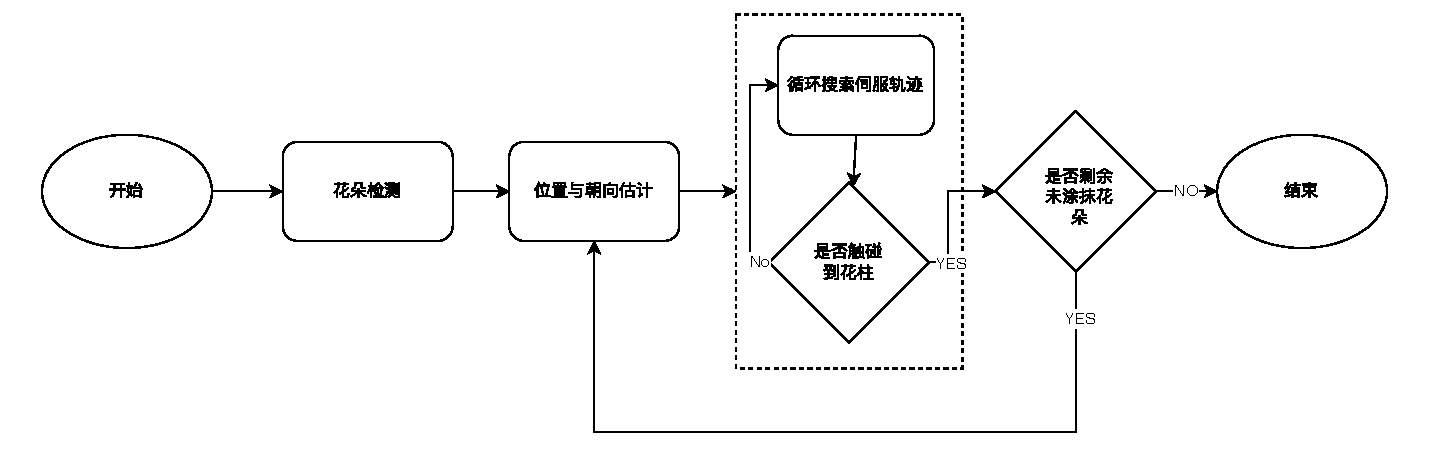
\includegraphics[width=1 \textwidth]{flowchat}
	\caption[柔顺授粉系统工作流程]{柔顺授粉系统工作流程} % 中括号中内容为插图索引中显示内容,可在题注内容过长时使用
	\label{fig:flowchat}
\end{figure}
本研究设计了一个本端到端的视觉引导柔顺授粉控制架构系统,其整体流程如\cref{fig:flowchat}所示。系统首先启动视觉感知模块,通过RGB-D相机对植物花朵进行实时采集,并基于\ref{dectection}和\ref{sec:rebuild}中的方法估计图像中所有花朵的空间位置及其朝向,将图像坐标转换为世界坐标,完成对待授粉花朵的三维定位与姿态估计。

获取到全部待授粉花朵的位置与姿态后,系统进入路径规划与分步控制阶段。首先通过插值路径控制策略,指引机械臂末端刷头从当前位置运动至目标花朵附近,完成粗略接近。此后,系统启动基于圆形搜索轨迹的精细伺服控制模块,根据待授粉花朵花柱中心点在图像平面中构造多个伺服点,逐个推进花粉刷完成柔顺接触。

在伺服过程中,系统实时采集末端视角图像,并调用Inception-v3图像分类网络判断是否完成雌蕊接触。若判定为“已触碰”,则标记当前花朵为“已授粉”,并判断是否仍有其他待处理花朵;若仍有剩余目标,则系统重新进入定位与控制循环;否则,流程终止。该流程实现了从花朵识别、空间感知、路径规划到触觉判断的全过程自动化控制,具备良好的柔顺性与任务闭环能力。


\subsection{两阶段伺服控制}
在实现精准授粉操作时,单纯依赖一次性定位完成花粉刷与雌蕊的接触存在较大不确定性,尤其是在自然环境下花朵存在微小摆动、定位误差以及执行器精度限制的情况下。为此,本研究提出一种粗到精的两阶段伺服控制策略,分别对应于“花朵接近”与“精细伺服”两个阶段,旨在提升授粉操作的柔顺性与鲁棒性。

在第一阶段中,系统根据视觉检测模块提供的雌蕊三维位置与姿态信息,计算出机械臂末端的目标位姿,并通过逆运动学求解机械臂的关节角度,使机械臂从当前位置平稳地移动到距离待授粉花柱一定安全距离处。在该阶段,花粉刷并不与待授粉花朵发生直接接触,而是通过一次全局路径规划将其引导至花朵附近,完成粗定位。

在完成初步定位后,系统进入第二阶段,即精细伺服控制阶段。在该阶段中,花朵与末端刷头已共同出现在相机视野中,系统利用检测到的雌蕊朝向信息对花粉刷进行旋转,使其姿态尽可能与雌蕊法向垂直,从而确保后续接触方向与授粉生理要求一致。随后,系统启动一种圆形搜索轨迹伺服策略,以覆盖可能存在的定位误差和花朵抖动带来的偏差。


\begin{figure}[htb]
	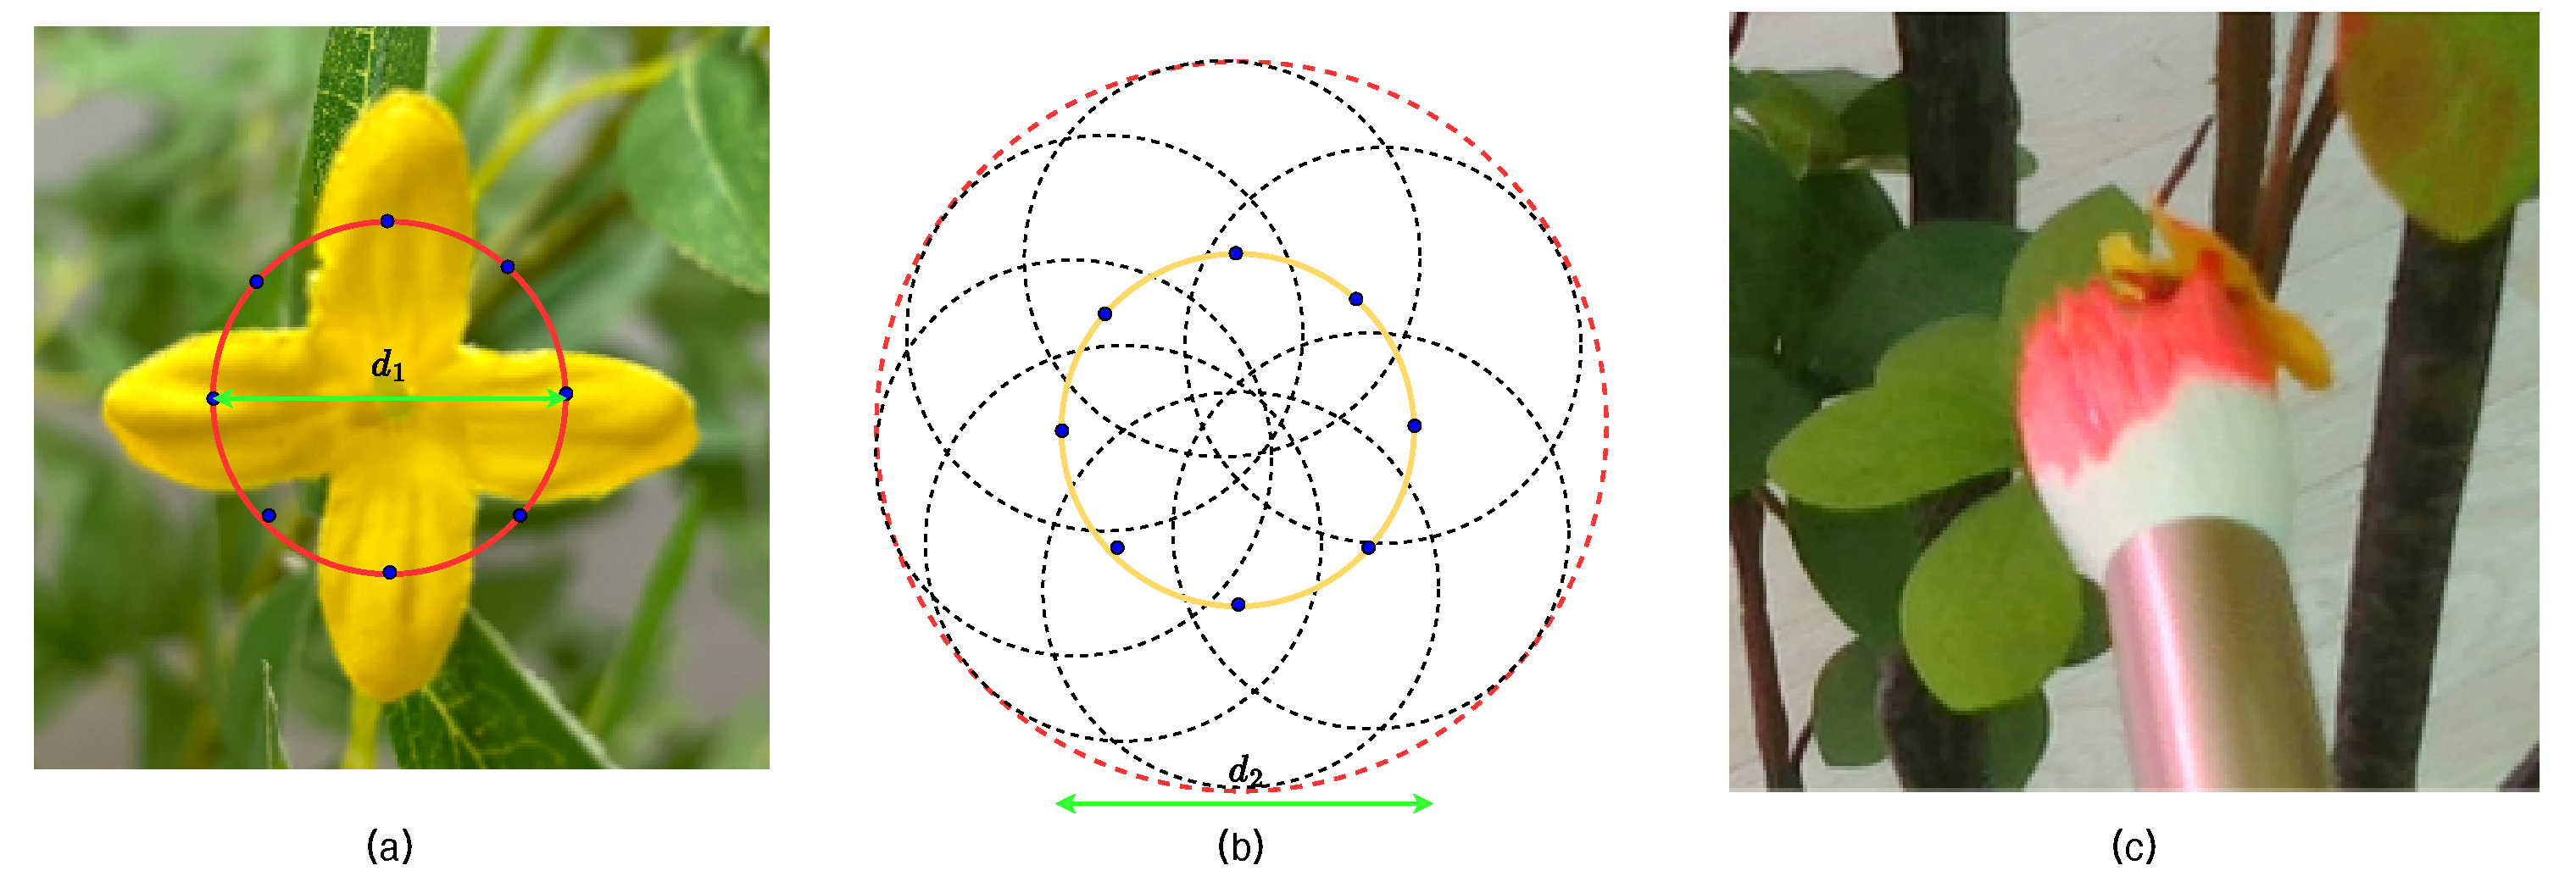
\includegraphics[width=1 \textwidth]{servoing}
	\caption[圆形搜索轨迹示意图]{圆形搜索轨迹示意图} % 中括号中内容为插图索引中显示内容,可在题注内容过长时使用
	\label{fig:servoing}
\end{figure}

圆形搜索轨迹伺服策略策略借鉴了Hanwen Kang提出的螺旋式伺服策略的思想,在待授粉花朵图像中心点的平面上构造一个大圆,并在其边缘等距布置八个伺服点,逐个依次控制花粉刷前进至这些点。\cref{fig:servoing}中(a)图中的红色大圆表示搜索路径,(b)图中黑色虚线表示搜索覆盖范围,此策略不仅在图像平面中进行二维伺服,还在三维空间中沿着垂直于花面方向长度为$K$,等间距布置多个圆轨迹层,构成一个圆柱形的伺服搜索体积,从而实现对雌蕊区域的空间覆盖。整个伺服空间体积可表示为:
\begin{equation}
	\label{equ:servoing_volum}
    V = \pi \cdot K \cdot d \cdot \frac{(d_{1}+d_{2})^{2}}{4}
\end{equation}

在伺服过程中,为了判断花粉刷是否已经成功接触到待授粉花朵,系统引入了图像识别模块,对当前相机视图进行分类。具体实现采用轻量级神经网络结构Inception-v3,对每一帧图像进行二分类,判断是否出现“已触碰”状态。一旦图像分类模型识别出刷头成功接触雌蕊,系统立即终止当前伺服动作,并将该花朵标记为“已授粉”,随后进入下一个待处理的目标花朵,\cref{fig:servoing}中(c)图表示已触碰状态。
这种粗到精的分级控制方式将全局路径优化与局部伺服精调有机结合,在保证作业效率的同时,显著提升了授粉的精确性与柔顺性,尤其适用于自然环境中具有高动态变化和复杂几何结构的植物授粉任务。

\subsection{基于三次样条插值的关节空间柔顺运动控制}
在机械臂执行授粉任务过程中,为了避免在目标切换时出现剧烈加速、减速带来的震动与力冲击,我们在“花朵接近”阶段引入了三次样条插值方法,用于生成平滑、连续的运动轨迹,确保系统整体的柔顺性和安全性。系统首先根据花朵空间位置估计模块提供的多个花朵位姿,利用TSP算法生成最优访问路径,然后将每对相邻花朵作为一段插值区间。在每一段区间中,系统以起点和终点的关节角度作为约束,根据\cref{equ:Cubic Spline Interpolation 2}构造三次样条插值函数。

插值轨迹的求解过程采用自然边界条件(即起止段加速度为0),通过构造并求解一个线性方程组,计算出每段插值曲线的系数。生成的轨迹再经过离散化处理,逐步下发到机械臂控制执行,最终驱动机械臂平稳地从当前花朵移动到下一朵花的附近位置,完成粗略接近。

这种插值策略在不依赖复杂优化算法的前提下,实现了对机械臂运动轨迹的高质量柔顺控制,特别适合在开放空间内进行的连续多目标作业场景。与伺服控制阶段形成互补,一方面负责大范围、低精度、连续性的轨迹生成,另一方面实现小范围、高精度、响应性的接触动作,共同构成完整的授粉控制闭环。

\section{实验设计与结果分析}
为了验证本章提出的基于插值轨迹与精细伺服策略的柔顺授粉控制方法的有效性,本文搭建了一个实际授粉实验平台,并在温室环境中对12株植物进行了多轮真实授粉测试。实验围绕机械臂在实际环境中对多朵花朵进行柔顺接近、伺服接触与结果评估展开,重点考察系统的任务完成率、操作精度、时间成本与算法表现。
\subsection{柔顺授粉实验环境搭建}
\begin{figure}[htb]
	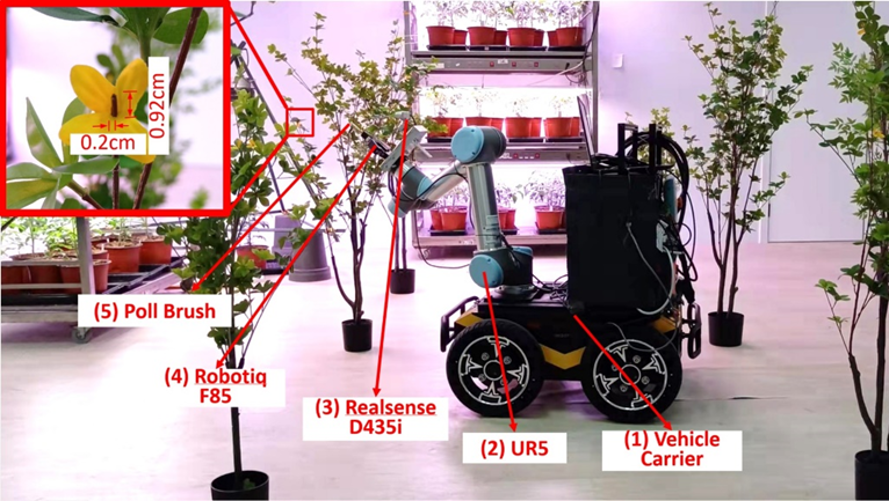
\includegraphics[width=1 \textwidth]{robot_env.jpg}
	\caption[柔顺授粉实验环境搭建]{柔顺授粉实验环境搭建} % 中括号中内容为插图索引中显示内容,可在题注内容过长时使用
	\label{fig:robot_env}
\end{figure}
为了验证本章提出的机械臂柔顺授粉控制方法的有效性,我们在室内环境下搭建了一个集感知、控制与执行于一体的授粉实验平台。该平台由移动底盘、机械臂、授粉末端、视觉感知系统以及控制计算单元等多个模块组成,具备在实际场景中完成自动化授粉任务的能力。

如\cref{fig:robot_env}所示,整个平台以MR1000 轮式移动机器人为基础构建。在平台上安装了一台 Universal Robots UR5 六自由度协作机械臂,其工作半径为 850 mm,最大负载为 5 kg,具备良好的空间覆盖性和运动灵活性,能够应对植物多样的开花方位与空间结构。UR5 的末端安装了 Robotiq F85 自适应夹爪,用于夹持柔软的羊毛材质花粉刷。该花粉刷形状为长 3.0 cm、直径 2.0 cm 的圆柱体,其末端连接有一个直径为 2.0 cm 的球状羊毛刷头,具备良好的生物兼容性与柔软接触特性,可有效避免在触碰花柱时对花朵造成损伤。为了实现视觉感知与闭环伺服控制,我们在机械臂末端安装了一台 Intel RealSense D453i RGB-D 相机,用于采集彩色图像与深度信息。该相机既用于在检测植物花朵的位置与朝向,也用于伺服控制阶段判断刷头是否接触到花柱,实现完整的视觉引导与反馈闭环。

系统的计算与控制单元由一台搭载 NVIDIA RTX 4050 显卡的便携式电脑组成,集成了多个感知与控制模块。其中包括用于花朵检测的模型、用于花柱方向识别的网络,以及用于触碰判别的分类网络,支持端到端自动化作业流程。该控制系统通过与机械臂驱动器的通信接口,实时下发插值轨迹与伺服指令,实现对多朵花朵的连续、柔顺授粉控制。
本实验采用的软硬件于下表中列出:
\begin{table}[htbp]
	\centering
	\caption[柔顺授粉控制软硬件]{柔顺授粉控制软硬件}
	\begin{tabularx}{\textwidth}{YYY}
		\toprule
		\textbf{序号} & \textbf{设备} & \textbf{型号} \\
		\midrule
		1 & 操作系统 & windows10 \\
		2 & cpu & intel13450X \\ 
		3 & 显卡 & NVIDIA GeForce RTX4050 \\
		4 & 运载底座 & MR1000 \\
		5 & 机械臂 & UR5 \\
		6 & 相机 & realsense \\
		7 & 夹爪 & Robotiq F85 \\
		8 & 授粉刷 & / \\
		9 & 授粉植株 & / \\
		\bottomrule
	\end{tabularx}
	\label{tab:pollination_env}
\end{table}
\subsection{实验设计}
为了系统验证所提出的基于插值与两阶段伺服控制的柔顺授粉方法的有效性,我们设计了对比实验,评估柔顺控制策略在实际应用中的表现提升程度。实验以是否采用柔顺控制策略作为主要对比变量,将系统分为两组:一组为对照组(未启用插值和伺服控制),另一组为实验组(采用本章提出的柔顺控制方法)。

实验场景设于室内环境,共布置12株植株,包含自然分布的121朵可授粉花朵。每组实验均在同环境中开展,确保目标花朵数量、空间分布、光照条件一致。每次试验过程中,机器人在完成对一株植物的检测、定位与路径规划后,依次对所有检测到的可授粉花执行授粉操作,并记录授粉成功率,授粉平均耗时指标。
其中,若刷头接触到花柱即记为“成功”,触碰花瓣但未触花柱记为“触碰未中”,完全未触及者记为“失败”。为客观评估授粉是否成功,我们使用蘸有红色颜料的花粉刷,通过残留痕迹判断是否成功接触花柱。
此外,我们分别记录系统中主要模块(花朵检测、花柱识别、位置转换、接近控制与伺服控制)的处理时间,并评估系统整体运行效率。
\subsection{结果与分析}
\begin{table}[htbp]
	\centering
	\caption[授粉结果]{授粉结果}
	\begin{tabularx}{\textwidth}{YYY}
		\toprule
		\textbf{评价指标} & \textbf{无柔顺控制} & \textbf{柔顺控制} \\
		\midrule
		授粉成功率(\%) & 82.3 & 96.5 \\
		总授粉次数(次) & 82 & 96 \\
		总尝试次数(次) & 158 & 112 \\
		平均每花尝试次数(次) & 1.58 & 1.12 \\
		单次授粉成功率(\%) & 51.9 & 85.7 \\
		单朵授粉耗时(s) & 30.1 & 18.9 \\
		\bottomrule
	\end{tabularx}
	\label{tab:pollination_env2}
\end{table}

\begin{figure}[htb]
	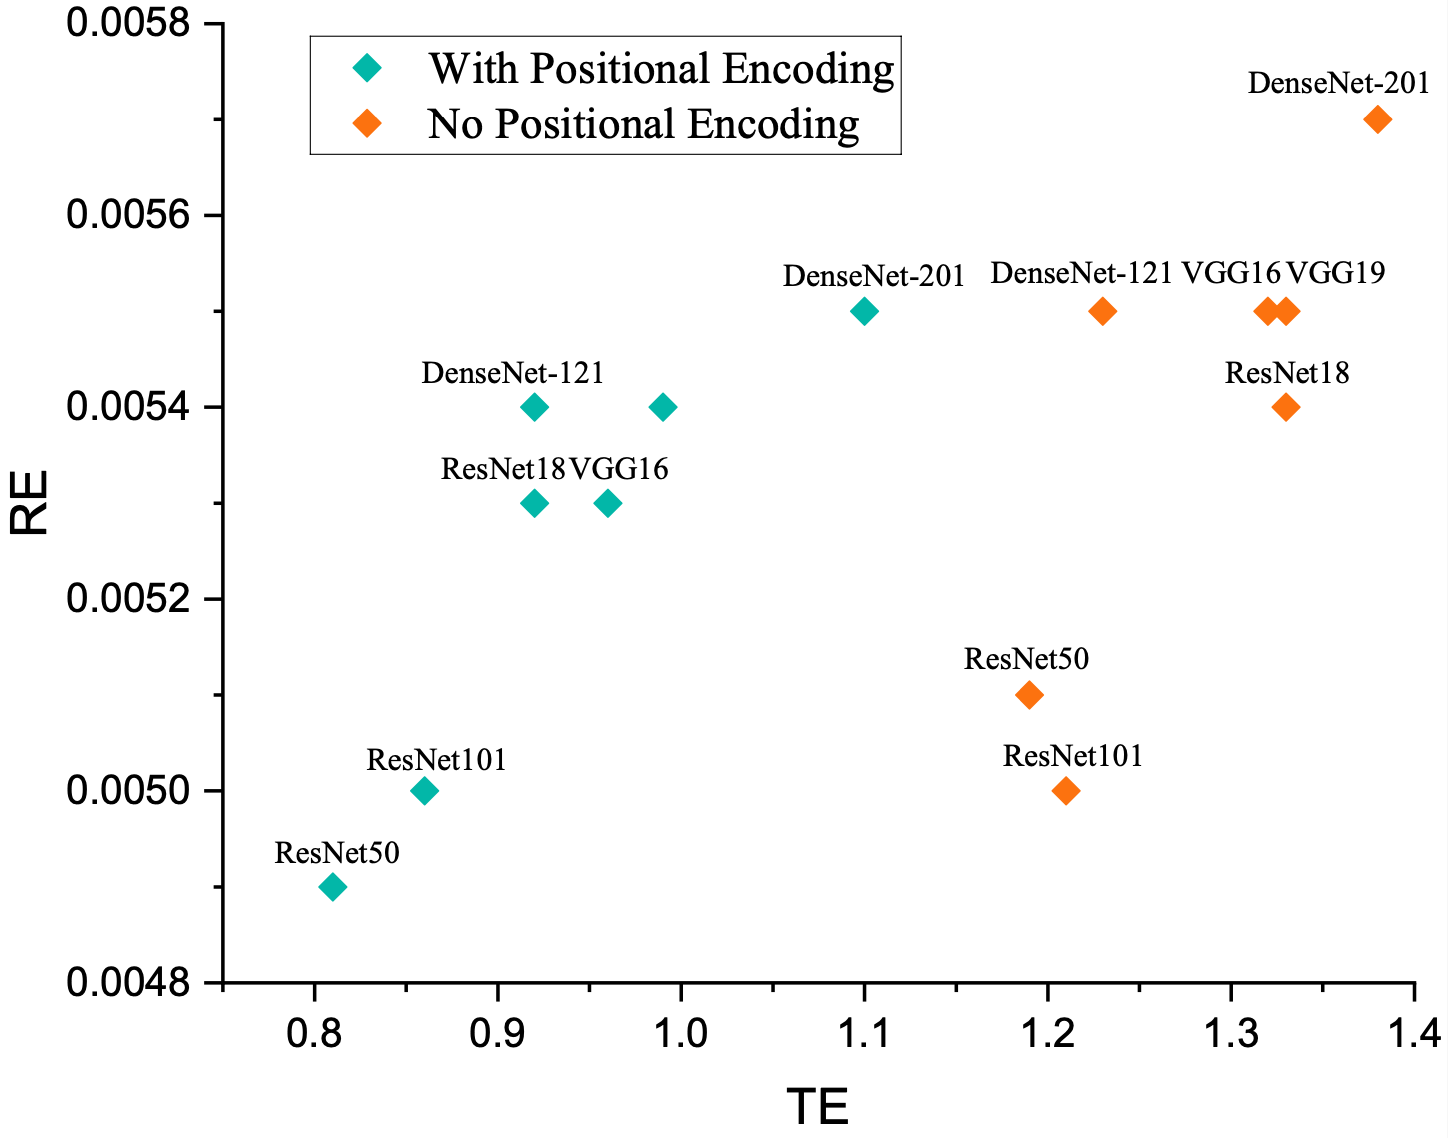
\includegraphics[width=1 \textwidth]{result}
	\caption[授粉实验结果主要指标对比]{柔顺控制实验结果主要指标对比} % 中括号中内容为插图索引中显示内容,可在题注内容过长时使用
	\label{fig:result4}
\end{figure}

从\cref{tab:pollination_env2}所列数据和\cref{fig:result4}显示结果可以看出,采用插值与两阶段伺服控制策略后,机械臂授粉系统在多个关键性能指标上均获得了显著提升。首先,在授粉效果方面,系统的授粉成功率由原始对照组的 82.3\% 提高至 96.5\%,说明插值路径与精细伺服策略有效提升了刷头与花柱之间的接触精度。同时,系统完成同样数量目标花朵的授粉所需的总尝试次数从 158 次下降至 112 次,平均每朵花的尝试次数由 1.58 次减少至 1.12 次,单次伺服成功率也从 51.9\% 提升至 85.7\%。这一变化表明,本方法在伺服过程中更为高效,命中率更高,减少了冗余伺服动作,有助于提升系统整体稳定性与节能性。

在系统执行效率方面,柔顺控制策略将单朵花的平均处理时间由 27.1 秒缩短至 18.9 秒,总任务耗时减少了约 30\%。这得益于插值方法在机械臂关节空间生成连续平滑的轨迹,使运动过程更加流畅,减少了运动过程中因关节越限而导致授粉无法继续的可能性。同时,视觉伺服阶段的快速定位与高命中率减少了重复调整的时间开销。

综合来看,插值与两阶段伺服控制策略的引入,在不增加系统结构复杂度的前提下,显著提升了机械臂在温室环境中的授粉能力。它不仅改善了机械臂的运动品质,也提升了系统的智能水平与任务闭环能力,为农业场景下的自动化操作提供了可靠支撑。该策略具备良好的通用性,适用于结构复杂、目标不确定性高的连续性操作任务。

\section{本章小节}
本章围绕授粉任务中对柔顺性的需求,提出并实现了一种基于三次样条插值与两阶段伺服控制相结合的柔顺运动控制策略。首先,设计了一个端到端的视觉引导柔顺授粉系统,整合花朵检测、三维定位、路径规划与触觉反馈模块,实现了完整的闭环控制流程。针对自然环境下花朵定位不确定性与微动干扰,提出粗到精的两阶段伺服控制方法,结合圆形搜索轨迹提升接触鲁棒性。为了保障机械臂大范围运动过程的平滑性与安全性,引入三次样条插值技术生成连续轨迹,显著减少了运动震动与误触风险。

实验部分在真实温室环境下验证了所提方法的有效性。与未采用柔顺控制的对照组相比,提出的方法在授粉成功率、单次伺服命中率、平均耗时等关键指标上均取得明显提升。其中授粉成功率提升至96.5\%,单花平均耗时缩短至18.9秒,体现出较强的实用性与推广价值。

